\documentclass[../main.tex]{subfiles}

\begin{document}

\begin{definition}
$V$ is a real vector space, an \textit{almost complex structure}\index{Almost complex structure} is an endomorphism $J:V\to V$ such that $J^2=-I$. Let $V^{1,0}\oplus V^{0,1}=V_{\mathbb C}$ be the $\pm i$ eigenspaces of $J$
\end{definition}

\begin{proposition}
We can find basis such that $V\cong \mathbb R^{2n}$ such that $J=\begin{pmatrix}
0&-I\\
I&0
\end{pmatrix}$. For local coordinate $(x_i,y_i)$ of a complex manifold, $\left\{\dfrac{\partial}{\partial x_i},\dfrac{\partial}{\partial y_i}\right\}$ is such a basis, $\dfrac{\partial}{\partial z_i},\dfrac{\partial}{\partial \bar z_i}$ are the $\pm i$ eigenvectors. This motivates the definition of a real isomorphism $\rho:V\to V^{1,0}$, $v\mapsto\dfrac{1}{2}(v-iJv)$, then $\rho J=i\rho$. Suppose $V,W$ both have almost complex structures, given an $\mathbb R$-linear map $T:V\to W$, let $\tilde T:V^{1,0}\to W^{1,0}$ be given by the commutative diagram
\begin{center}
\begin{tikzcd}
V \arrow[r, "T"] \arrow[d, "\rho"'] & W \arrow[d, "\rho"] \\
{V^{1,0}} \arrow[r, "\tilde T"]     & {W^{1,0}}          
\end{tikzcd}
\end{center}
$\tilde T$ is complex linear if $TJ=JT\iff\tilde T i=i\tilde T$. Alternatively, extend $T$ to a map $V_{\mathbb C}\to W_{\mathbb C}$, and this conditions is exactly that this extension preserves $(1,0)$ and $(0,1)$ subspaces
\end{proposition}

\begin{lemma}[Osgood's lemma]
If $f:\Omega\to\mathbb C$ is continuous and holomorphic in each variable, then it is analytic
\end{lemma}

\begin{proof}
Iterate Cauchy's formula and use Fubini's theorem to write
\[f(z)=\left(\frac{1}{2\pi i}\right)^n\int_{w_i\in\Delta(z_i,r_i)}\frac{f(w)dw}{(w_1-z_1)\cdots(w_n-z_n)}\]
Then
\[\frac{1}{(w_1-z_1)\cdots(w_n-z_n)}=\sum_I\frac{(z-\xi)^I}{(w-\xi)^I}\]
Then a convergent power series expression follows, with
\[c_I\left(\frac{1}{2\pi i}\right)^n\int_{w\in\Delta(z,r)}\frac{f(w)dw}{(w_1-z_1)^{i_1+1}\cdots(w_n-z_n)^{i_n+1}}\]
The \textit{total order} of an analytic function $f$ at $\xi$ is the smallest value of $|I|$ for which $c_I\neq0$
\end{proof}

\begin{definition}
A set $E\subseteq\Omega$ is called \textit{thin} if for every $\xi\in E$ there is a polydisk $\Delta(\xi,r)\subset\subset\Omega$ and $g\in A(\Delta(\xi,r))$ such that $E\cap\Delta(\xi,r)\subseteq Z(g)$. Note that for $n=1$, this is equivalent to discrete
\end{definition}

\begin{theorem}[Riemann extension theorem]
If $f\in A(\Omega\setminus E)$ where $E$ is a thin set, and $f$ is locally bounded on $\Omega$, then there exists $\tilde f\in A(\Omega)$ such that $\tilde f=f$ on the complement of $E$
\end{theorem}

\begin{proof}
Let $k$ be the total order of $g$ at $\xi$. By an application of Rouch\'e's theorem (and after modifying $r$ and a change of variables), we can assume that for each $z_1,\cdots,z_{n-1}$ the function $z_n\mapsto g(z_1,\cdots,z_{n-1},z_n)$ has exactly $k$ zeros and none on the boundary
\end{proof}

In higher dimensions, to solve $\bar\partial$ equation, there must be a \textit{integrability condition}. Indeed, if we can solve the equation, then $0=\bar\partial^2u=\bar\partial\alpha$, i.e. we require $\alpha$ to be $\bar\partial$ closed

\begin{proposition}
Let $n\geq2$. If $\alpha$ is a smooth compactly supported $(0,1)$ form on $\mathbb C^n$ with $\bar\partial\alpha=0$, then there is a $u\in C_c^\infty$, with $\bar\partial u=\alpha$
\end{proposition}

\begin{proof}

\end{proof}

\begin{corollary}[Hartogs theorem]
Let $K\subseteq\Omega$ be compact with $\Omega\setminus K$ connected. If $f\in A(\Omega\setminus K)$, there exists $\tilde f\in A(\Omega)$ that is equal to $f$ on the complement of $K$
\end{corollary}

\begin{proof}
Let $\phi\in C_c^\infty(\Omega)$ be $\equiv1$ in a neighborhood of $K$, let $\alpha=\bar\partial((1-\phi)f)$. Then $\alpha$ is $\bar\partial$-closed and compactly supported. Hence, there is $u\in C_c^\infty(\mathbb C^n)$ with $\bar\partial u=\alpha$. Then let $\tilde f=(1-\phi)f-u$, $\tilde f\in A(\Omega)$, since $u$ is compactly supported, $\tilde f=f$ on $\Omega\setminus K$
\end{proof}

\begin{note}
The assumption that $\Omega\setminus K$ is connected is necessary. For example, let $K\subseteq B(0,1)=\{|z|<1\}$ be the set where $|z|=\frac{1}{2}$, and take
\[f(z)=\begin{cases}
z_n &\text{if }1/2<|z|<1 \\
0 &\text{if }|z|<1/2
\end{cases}\]
Then there is no holomorphic extension to $B(0,1)$
\end{note}

\begin{proposition}
If $\alpha$ is a smooth $\bar\partial$-closed $(0,1)$ form on a polydisk $\Delta=\Delta(0,r)$, then $\alpha=\bar\partial u$ for some $u\in C^\infty(\Delta)$
\end{proposition}

\begin{proof}
Just like in the one variable case, exhaust $\Delta$ by nested closed polydiscs $K_i$. Use cut-off functions to find $u_i$, $\bar\partial u_i$ in a neighborhood of $K_i$. Then $u_{i+1}-u_i$ is holomorphic in a neighborhood of $K_i$. Now by the power series expansion, there is a polynomial $p_i$ such that $\|u_{i+1}-u_i-p_i\|_{K_i}<2^{-i}$. The rest follows as in the proof of the one variable case
\end{proof}

\begin{note}
We heavily used the geometric properties of the polydisc
\end{note}

\begin{corollary}[Cousin theorem]
$\mathcal U=\{u_i\}$ is an open cover of polydisc $\Delta$, then $H^1(\Delta,\mathcal U)=0$
\end{corollary}

\begin{theorem}
If $\alpha\in C^\infty_{(p,q)}(\Delta)$, $q\geq1$, $\bar\partial\alpha=0$. Then $\alpha=\bar\partial u$ for some $u\in C^\infty_{(p,q-1)}(\Delta)$
\end{theorem}

\begin{remark}
This states that the Dolbeault cohomology groups $H^{p,q}_{\bar\partial}(\Delta)=0$
\end{remark}

\begin{proof}
Induct on $k=1,\cdots,n$, the smallest integer such that $\alpha$ only involves $d\bar z_1,\cdots,d\bar z_k$. If $k=1$, then $q=1$ and we have already proven the result. Suppose the result is true for $k-1$. Write $\alpha=\omega\wedge d\bar z_k+\beta$, where $\omega$ and $\beta$ only involve $d\bar z_1,\cdots,d\bar z_{k-1}$. We have $0=\bar\partial\alpha=\bar\partial\omega\wedge d\bar z_k+\bar\partial\beta$. This implies both $\omega,\beta$ are holomorphic in the variables $z_{k+1},\cdots,z_n$. Apply the one variable solution to find $\mu$, $\bar\partial\mu=\omega\wedge d\bar z_k+\sigma$, here $\sigma$ only involves $d\bar z_1,\cdots,d\bar z_{k-1}$. Now $\alpha-\bar\partial u=\beta-\sigma$ is $\bar\partial$-closed. By induction, we can write $\beta-\sigma=\bar\partial v$, and so we set $u=v+\mu$
\end{proof}

\begin{example}
Let $\Omega\subseteq\mathbb C^2$ be a domain. For $\xi\in\Omega$, let $\Omega^*=\Omega\setminus\{\xi\}$. Then $H^{0,1}_{\bar\partial}(\Omega^*)\neq\{0\}$
\end{example}

\begin{proof}
Without loss of generality assume $\xi=(0,0)$. Consider the $(0,1)$-form
\[\omega=\frac{1}{r^4}(-\bar z_2d\bar z_1+\bar z_1d\bar z_2)=\bar\partial\left(\frac{\bar z_2}{z_1r^2}\right)\]
Clearly, $\omega$ is smooth on $\Omega^*$, and $\bar\partial\omega=0$. Suppose $\omega=\bar\partial u$ for $u\in C^\infty(\Omega^*)$. Then $f(z_1,z_2)=z_1u-\dfrac{\bar z_2}{r^2}$ is holomorphic on $\Omega^*\setminus\{z_1=0\}$, and it is locally bounded on $\Omega^*$. By Riemann extension, it is holomorphic on $\Omega^*$. By Hartogs, it extends to $\Omega$. But for $z_2\neq0$ we clearly have $f(0,z_2)=-\dfrac{1}{z_2}$, contradiction
\end{proof}

\begin{proposition}
$K\subseteq\Omega$ is compact
\begin{enumerate}
\item $\hat K_\Omega$ is closed in $\Omega$
\item $\hat K_\Omega$ is not necessarily closed in $\mathbb C^n$. E.g. if $n\geq2$, let $\Omega=\mathbb B^n\setminus\{0\}$, $K=\{|z|=1/2\}$. Then by Hartogs' theorem, $\hat K_\Omega=\mathbb B^n_{1/2}\setminus\{0\}$
\item $\hat K_\Omega\subseteq\mathcal C(K)$, the closed convex hull of $K$. In particular, $\hat K_\Omega$ is bounded
\end{enumerate}
\end{proposition}

\begin{proof}
Let $w\notin\mathcal C(K)$, $z_0\in\mathcal C(K)$ minimizes distance to $w$, let $\xi\in(\mathbb C^n)^*$ define a supporting hyperplane for $\mathcal C(K)$ so that $\mathcal C(K)\subseteq\Re\langle\xi,z\rangle\leq0$ and $\Re\langle\xi,w\rangle\geq0$. Let $f(z)=\exp\langle\xi,z\rangle$, $|f(z)|=\exp\Re\langle\xi,z\rangle$ which violates the definition, so $w\notin\hat K_\Omega$
\end{proof}

\begin{definition}
A domain $\Omega\subseteq\mathbb C^n$ is \textit{holomorphically convex}\index{holomorphically convex} if for every compact $K\subseteq\Omega$, $\hat K_\Omega$ is compact. If $\Omega$ is convex, then it is holomorphically convex. If $n=1$, all domains are holomorphically convex. The previous counter-example shows this is not true if $n\geq2$
\end{definition}

\begin{proposition}
$\Omega\subseteq\mathbb C^n$ is holomorphically convex $\iff$ every discrete, infinite set $\{z_j\}\subseteq\Omega$ there is $f\in A(\Omega)$ with $|f(z_j)|$ unbounded
\end{proposition}

\begin{proof}
$\Leftarrow$: If $\hat K_\Omega$ is not compact there is a discrete infinite subset $\{z_j\}\subseteq\hat K$. But then $|f(z_j)|\leq\|f\|_K$, $\forall j,f\in A(\Omega)$. This contradicts the existence of $f\in A(\Omega)$ where $|f(z_j)|$ is unbounded
\begin{center}
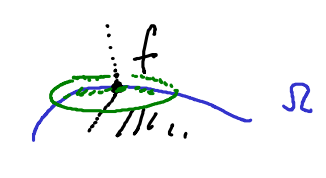
\includegraphics[scale=1]{Pictures/Holomorphic_convexity.png}
\end{center}
$\Rightarrow$: Exhaust $\Omega$ by nested compact sets $K_j$, $\hat K_j=K_j$. We may assume $z_j\in K_{j+1}\setminus K_j$. We can find $f_j\in A(\Omega)$ such that $f_j(z_j)=1$, $\|f_j\|_{K_j}<1$, by taking power, $\|f_j\|_{K_j}$ can actually be arbitrarily small. Let $g_j\in A(\Omega)$ be such that $g_j(z_j)=1$, $g_j(z_j)=0$ for $i<j$. Now define $\lambda_j$ by
\[\lambda_j=j-\sum_{i=1}^{j-1}\lambda_ig_if_i(z_j)\]
Assume $\|\lambda_jg_jf_j\|_{K_j}<2^{-j}$. Now let $f(z)=\sum_{i=1}^\infty\lambda_ig_if_i(z)$. This converges uniformly on compact sets, and so $f\in A(\Omega)$. Finally
\[f(z_j)=\sum_{i=1}^j\lambda_ig_if_i(z_j)=\lambda_jg_jf_j(z_j)+\sum_{i=1}^{j-1}\lambda_ig_if_i(z_j)=j\]
\end{proof}

\begin{definition}
$\Omega\subseteq\mathbb C^n$ is called a \textit{domain of holomorphy} if there is $f\in A(\Omega)$ such that for any $p\in\overline\Omega\setminus\Omega$ and any $\Omega'$ about $p$, there is no $g\in A(\Omega')$ such that $g=f$ on $\Omega'\cap\Omega$
\end{definition}

\begin{theorem}
$\Omega\subseteq\mathbb C^n$ is holomorphically convex $\iff$ it is a domain of holomorphy
\end{theorem}

\begin{corollary}
A convex domain in $\mathbb C^n$ is a domain of holomorphy
\end{corollary}

\begin{proof}
$\Rightarrow$ is similar to the one variable case. $\Leftarrow$ is a theorem of Oka (this will be generalized) \\
$\Rightarrow$: Fix a polydisc $\Delta$ about the origin. For $\xi\in\Omega$, let $\Delta_\xi=\xi+r\Delta$, where $r$ is the supremum such that $\xi+r\Delta\subseteq\Omega$. Let $E\subseteq\Omega$ be countable dense. Let $\{\xi_j\}$ be a sequence containing every point of $E$ infinitely may times. Write $\Omega=\bigcup K_j$. Since $\hat K_j\subset\subset\Omega$, $\exists z_j\in\Delta_{\xi_j}$ with $z_j\notin\hat K_j$. Choose $f_j\in A(\Omega)$, $f_j(z_j)=1$, $\|f_j\|_{K_j}<2^{-j}$. Set $f(z)=\prod(1-f_j)^j$. Then $f$ converges uniformly on compact sets, so $f\in A(\Omega)$. Now $f$ has zeros of order $\geq j$ at $z_j$. Any continuation of $f$ would have a zero of infinite order \\
$\Rightarrow$: Let $d(z)=\sup_{\Delta(z,r)\subseteq\Omega}r$, $d(K)=\inf_{z\in K}d(z)$. Claim $d(\hat K)=d(K)>0$. This will imply $\hat K\subset\subset\Omega$. Let $f\in A(\Omega)$ so that the radius of convergence at $z$ is $d(z)$, let $\delta <d(K)$, $K_\delta=\bigcup_{w\in K}\overline{\Delta(w,\delta)}$. By Cauchy estimates: $\|D^If\|_K\leq\dfrac{I!}{\delta^{|I|}}\|f\|_{K_\delta}$. But $D^If\in A(\Omega)$, so for $z\in\hat K$, $|D^If(z)|\leq\|D^If\|_K\leq\dfrac{I!}{\delta^{|I|}}\|f\|_{K_\delta}$. This implies that the radius of convergence at $z\in\hat K$ is at least $\delta$, i.e. $d(z)\geq\delta$, and so $d(\hat K)\geq d(K)$. Since $K\subseteq \hat K$, the other inequality is trivial
\end{proof}

\begin{proposition}
If $\{\Omega_\alpha\}_{\alpha\in I}$ are domains of holomorphy in $\mathbb C^n$, then the interior $\Omega$ of $\bigcap_{\alpha\in I}\Omega_\alpha$ is also a domain of holomorphy
\end{proposition}

\begin{proof}
$K\subseteq\Omega$ is compact. For each $\alpha\in I$, $K\subseteq\Omega\subseteq\Omega_\alpha$, which implies $\hat K_\Omega\subseteq\hat K_{\Omega_\alpha}$. This implies $d_{\Omega_\alpha}(\hat K_{\Omega_\alpha})\leq d_{\Omega_\alpha}(\hat K_\Omega)$, for all $\alpha$. Since $\Omega_\alpha$ is holomorphically convex, $d_{\Omega_\alpha}(\hat K_{\Omega_\alpha})=d_{\Omega_\alpha}(K)$. Hence $d_\Omega(K)\leq d_{\Omega_\alpha}(K)\leq d_{\Omega_\alpha}(\hat K_\Omega)$. Finally, this implies $d_\Omega(K)\leq d_\Omega(\hat K_\Omega)$. As before, we conclude that $d_\Omega(K)=d(\hat K_\Omega)$, and so $\hat K_\Omega$ is compact, so $\Omega$ is holomorphically convex
\end{proof}

\begin{claim}
Suppose $\Omega$ is a domain of holomorphy. Let $f_1,\cdots,f_N\in A(\Omega)$, and define
\[\Omega_c=\{z\in\Omega||f_j(z)|<c,j=1,\cdots,N\}\]
Then $\Omega_c$ is also a domain of holomorphy
\end{claim}

\begin{proof}
Let $K\subseteq\Omega_c$. Let $z\in\hat K_\Omega$. Then in particular, for any $j=1,\cdots,N$, $|f_j(z)|\leq\|f_j\|_K<c$. So $z\in\Omega_c$. Now $\hat K_{\Omega_c}\subseteq\hat K_\Omega\subseteq\Omega$ and so $\hat K_{\Omega_c}$ is compact
\end{proof}

\begin{claim}
Let $u:\Omega\subseteq\mathbb C^n\to\mathbb C^m$ be holomorphic, with $\Omega$ a domain of holomorphy. If $\Omega'\subseteq\mathbb C^m$ is a domain of holomorphy, then so is $\tilde\Omega=u^{-1}(\Omega')$
\end{claim}

\begin{proof}
Let $K\subseteq\tilde\Omega\subseteq\Omega$ be compact. Since $\hat K_{\tilde\Omega}\subseteq\hat K_\Omega\subseteq\Omega$, it suffices to show $\hat K_{\tilde\Omega}$ is closed in $\Omega$. Let $z_j\to z\in\Omega$, $z_j\hat K_{\tilde\Omega}$. Notice that $u(\hat K_{\tilde\Omega})\subseteq\widehat{u(K)}_{\Omega'}$. Hence $u(z)\in\Omega'$, and so $z\in\tilde\Omega$
\end{proof}

\begin{lemma}
Let $\Omega\subseteq\mathbb C^n$ be a domain of holomorphy, and $K\subseteq\Omega$. Suppose $f\in A(\Omega)$ is such that $|f(z)|\leq d(z)$ for all $z\in K$, then $|f(\xi)|\leq d(\xi)$ for all $\xi\in\hat K_\Omega$
\end{lemma}

\begin{proof}
We first claim that if $u\in A(\Omega)$, then the power series expansion of $u$ at $\xi\in\hat K_\Omega$ converges on $\Delta(\xi,|f(\xi)|)$. This will prove the Lemma, because we can take $u$ to be teh function with no analytic continuation beyond $\Omega$ \\
Proof of the claim: Let $0<\delta<1$, as before, the Cauchy estimates provide for some constant $M$ that
\[|D^Iu(z)|\frac{(\delta|f(z)|)^{|I|}}{I!}\leq M,\forall z\in K\]
Now $D^Iu(z)f(z)^{|I|}\in A(\Omega)$, so the same estimate holds on $\hat K_\Omega$. This means the radius of convergence at $\xi\in \hat K_\Omega$ is a t least $\delta|f(\xi)|$. Since $\delta$ was arbitrary, this proves the claim
\end{proof}

Fundamental consequence: Let $D\subset\subset\Omega$ be a 1-dimensional disc
\begin{enumerate}
\item Suppose $f$ is a polynomial in one variable such that $-\log d(z)\leq\Re f(z)$, for $z\in\partial D$
\item Let $f$ be the restriction of $F\in A(\Omega)$. Then $|e^{-F(z)}|\leq d(z)$, $z\in\partial D$
\item By the maximum principle, $D\subseteq\widehat{\partial D_\Omega}$
\item From the Lemma, we have $|e^{-F(z)}|\leq d(z)$, $z\in\partial D$
\item This in turn implies $-\log d(z)\leq\Re f$ on $D$
\end{enumerate}
Approximating harmonic functions by polynomials, we conclude that $u=-\log d$ is subharmonic on any complex line in $\Omega$

\end{document}